\selectlanguage{ngerman}
\begin{abstract}
In der Videospiel- und Animationsfilmindustrie spielen 3D-Modelle eine zentrale Rolle. 
Sie bieten einem Künstler die Möglichkeit Charakteren und Umgebungen zu modellieren, die eine Darstellung der Realität simulieren soll. \newline
In der Computergrafik sind Dreiecksnetzes eine gängige Datenrepräsentation von 3D-Modellen. 
Die Modelle werden jedoch immer komplexer, was den Speicherbedarf erhöht und die zur Darstellung benötigte Zeit verlängert. Um diesen Anforderungen gerecht zu werden, müssen neue Methoden zur Datenkompression entwickelt werden. Ziel dieser Arbeit ist es, ein Verfahren zu entwickeln, um ein komprimiertes Dreiecksnetz in die GPU zu laden und dort zu dekodieren. Insbesondere sollen das Kompressionsverhältnis, Dekompressionsrate und visuelle Qualität quantitativ untersucht und auswertet werden. Die Ergebnisse dieser Arbeit werden, wenn möglich, mit den Resultaten von gängigen Kompressionsmethoden verglichen.
\end{abstract}
\selectlanguage{english}
\begin{abstract}
3D models play a central role in the video game and animation film industry. 
They offer artists the opportunity to model characters and environments that simulate a representation of reality. \newline
In computer graphics, triangle meshes are a common data representation of 3D-models. 
However, the models are becoming increasingly complex, which increases the memory requirements and extends the time needed for visualisation. To meet these requirements, new methods for data compression must be developed. The aim of this work is to develop a method for loading a compressed triangle mesh into the GPU and decoding it there. In particular, the compression ratio, decompression rate and visual quality are to be quantitatively analysed and evaluated. If possible, the results of this work will be compared with the results of common compression methods.
\end{abstract}
\selectlanguage{ngerman}
\section{Einführung}
In der Computergrafik ist die Erzeugung eines Dreiecksnetzes eine gängige Methode zur Generierung von 3D-Modellen. Diese Modelle können in Topologie und Geometrie unterteilt werden. Für die Geometrie werden verschiedene Attribute benötigt. 
So werden die Positionen, die Normalen und Texturkoordinaten/Farbwerte für jeden Punkt des Dreiecksnetzes in 32 Bit Gleitkommazahlen gespeichert. 
Für die korrekte Anordnung und Reihenfolge der Knotenpunkte ist die Topologie zuständig. 
Dabei ist die Datenkompression ein entscheidendes Thema. 
In einer Welt, in der digitale Daten schon lange ein wichtiges Thema sind und dennoch immer weiter an Bedeutung gewinnen, ist die effiziente Speicherung und Übertragung ein wichtiger Gesichtspunkt.
3D-Modelle werden so gut wie überall benötigt. 
Videospiele und Animationsserien wären ohne nicht vorstellbar. 
Architekten können ihre Ideen auch ohne Bleistift auf das Papier (oder den Bildschirm) bringen.
Künstler wollen Modelle erschaffen, die den Eindruck gewinnen wollen, realitätsgetreu zu sein. 
Die Folge davon ist, dass diese Modelle stetig komplexer werden und somit ein größerer Speicheraufwand benötigt wird. 
Um dem entgegenzuwirken, werden Methoden verwendet, diese digitalen Informationen zu komprimieren.

\subsection{Geschichtlicher Hintergrund der Datenkompression}
\label{subsec:main_kompression}
Ursprünglich zur Repräsentation von Daten entwickelt, wurde der Morse Code zu einem der wichtigsten Werkzeuge für die Kommunikation des 19. Jahrhunderts. 
Bestehend aus zwei Grundbausteinen, einem kurzen und einem langen Signal, konnten einzelne Buchstaben kodiert werden. 
Erweitert man dieses Alphabet mit einem weiteren Symbol, einer Pause, die zwischen einzelnen Signalsequenzen eingelegt wird, können ganze Wörter und Sätze übermittelt werden. 
Das bekannteste Werkzeug für den Morse Code ist der Telegraf, mit dem diese Signale über weite Strecken übertragen werden konnten.
Die Erfindung des Morsecodes findet im 21. Jahrhundert nicht nur seinen Zweck in dramatischen Momenten des in Film und Fernsehens. 
Es war zeitgleich ein früher und großer Meilenstein und Wegbegleiter für die Kompression einer Datenquelle (in diesem Fall des Alphabets). 
Durch Untersuchungen einer großen Anzahl an Literatur kann eine Buchstabenhäufigkeit berechnet werden. 
Diese sagt aus, wie wahrscheinlich es ist, welcher Buchstabe in einem Text folgt, ohne den aktuellen Kontext, in Form von vorgehenden Buchstaben, zu betrachten.
Da die Wahrscheinlichkeit eines Zeichens abhängig vom Alphabet ist, sollten diese nicht übergreifend für andere Alphabete verwendet werden. 
So sind die Buchstaben \glqq E\grqq\ und \glqq T\grqq\ die Buchstaben des englischen Alphabets, welche die höchste Auftrittswahrscheinlichkeit besitzen, während sich im deutschen Alphabet der Buchstabe \glqq E\grqq\ von der Masse abhebt.
Der Morse Code hat gezeigt, welchen Nutzen die Kompression von Information beinhaltet.
Zu Kriegszeiten hat dieser eine effiziente und schnelle Übermittlung von Informationen ermöglicht.
Dadurch konnte in Krisenmomenten schnell reagiert werden, um so größeren Katastrophen frühzeitig abzuwenden, aber leider auch, solche zu verursachen.

\subsubsection*{Der Ist-Stand}
Springen wir in die heutige Zeit, sehen wir die Vorteile von komprimierten Daten in der modernen Welt.
Die meisten Menschen denken an JPEG und PNG, wenn sie an digitale Bilder denken.
Bekanntere Videoformate sind MP4, AVI und FLV.
Bei all diesen Formaten handelt es sich um komprimierte Rohdaten.
Das Filesystem eines jeden in der Industrie verwendeten Betriebssystems komprimiert diese Speichern von Daten automatisch.
Zusätzlich dazu besteht noch die Möglichkeit, seine Daten manuell zu komprimieren mithilfe von Programmen wie 7-Zip, WinRar oder WinZip.
Datenkompression kann in so gut wie allen Bereichen angetroffen werden.
Und die Gründe dafür sind simpel.
Speicherplatz ist teuer, und das Ressourcenmanagement wird deutlich vereinfacht, wenn die benötigte Hardware minimiert wird.
Betrachten wir das Streamen von Daten auf dem Beispiel des größten Videostreaming-Dienstes YouTube.
Laut Statistiken werden pro Minute hunderte Stunden an Videomaterial hochgeladen, Tendenz steigend (siehe Abbildung \ref{fig:youtube}).
\begin{figure}[htb]
  \centering  
  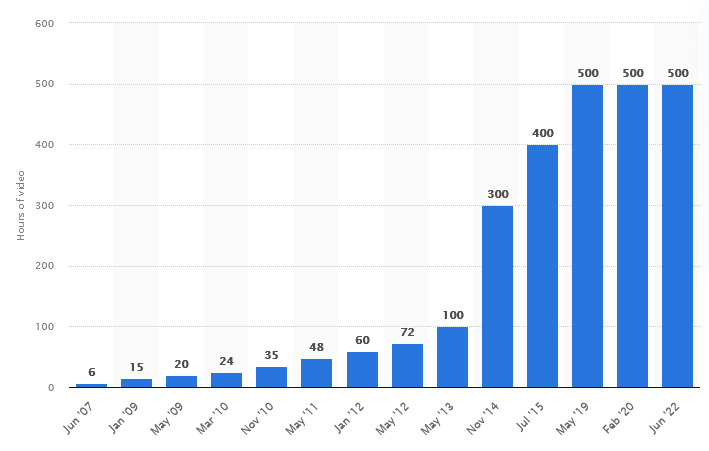
\includegraphics[scale=0.8]{Bilder/youtube_statistik.png}
  \caption[YouTube Statistik]{\textbf{Anzahl der YouTube-Videos} Die Anzahl an Minuten, die auf YouTube hochgeladen werden.
  Abbildung von Statista: https://www.statista.com/statistics/259477/hours-of-video-uploaded-to-youtube-every-minute/ }
  \label{fig:youtube}
\end{figure}
Um die Unmengen an Videos zu speichern, benötigt Google riesige Serverfarmen, die auf dem gesamten Globus verstreut sind.
Eine genaue Zahl ist der Öffentlichkeit nicht bekannt, es steht jedoch außer Frage, dass diese nochmal um einiges höher ausfällt, würden die Daten nicht komprimiert werden. \newline

Ein weiterer Aspekt ist der eigentliche Nutzen von YouTube, nämlich das Abspielen von Videos.
Um ein Video sehen zu können, muss es vom YouTube-Server dem Client übertragen werden.
Durch die Komprimierung der Quelldateien sind die zu übertragenden Daten schon geschrumpft.
Es können jedoch noch weitere Schritte absolviert werden, um die Daten für den Nutzer besser zugänglich zu machen.
Dazu werden Verfahren wie Trancoding, Transsizing und Transrating verwendet.
Transcoding beschreibt den Prozess, ein bereits komprimiertes Videoformat in ein anderes, eventuell für den Client besser zugeschnittenes Videoformat zu komprimieren.
Das sollte jedoch nicht zu oft angewendet werden, da die Qualität beim wiederholten Komprimieren und Dekomprimieren verloren geht; sollten die Verfahren verlustbehaftet sein. \newline
In vielen Fällen kann die originale Auflösung vom Endgerät nicht abgespielt werden und wird deshalb von diesem auf eine niedrigere Auflösung skaliert.
Beispielsweise wenn das Endgerät lediglich 1080p auflösen kann, aber ein Video in einer Auflösung von 4K wiedergegeben werden soll.
Trotzdem werden die vollen Daten des Videoformats empfangen.
Um diese Verschwendung von Bandbreite zu sparen, wird Transsizing verwendet.
Die originalen Daten werden in eine kleinere Auflösung skaliert und anschließend übertragen. \newline
Um die Bitrate zu minimieren, wird Transrating verwendet.
So kann die Auflösung bei geringerer Bitrate beibehalten werden.
Die Verfahren zur Minimierung des Datenstroms hören sich zunächst sehr mächtig an, sind jedoch mit Vorsicht zu genießen.
Der Vorgang ist nämlich verlustbehaftet und kann bei zu starker Nutzung zu Artefakten führen.
Dafür ermöglicht es jedoch Menschen, deren Internetzugang ein Abspielen in hoher Qualität nicht zulässt, den Streaming-Anbieter zu nutzen. \newline

Neben dem Beispiel von Streaming Anbietern reihen sich noch viele weitere Beispiele, die einen riesigen Vorteil von der Datenkompression ziehen.
In einem jedem BWL Grundlagenfach wird die Wichtigkeit des Wettbewerbsvorteils vermittelt.
Ein Unternehmen muss auf Marktveränderungen schnellstmöglich erkennen.
Insbesondere Unternehmen im Finanzbereich sind davon abhängig, damit die Datenanalyse schnellstmöglich auf Kursschwankungen reagieren kann.

\subsection{Steigende Komplexität}
\label{subsec:steigende_komplexität}
Das Beispiel der Unterhaltungsbranche hat aufgezeigt, warum Kompression in unserer heutigen Gesellschaft eine große Rolle spielt.
Um die Relevanz von Kompressionsalgorithmen in dem Kontext von Dreiecksnetzen aufzuzeigen, kann sich ein Beispiel an Videospielen genommen werden.
Physische Medien waren zu Beginn des 21. Jahrhunderts der Standard, um eine Form der Unterhaltung in den Haushalt zu bekommen.
Sei es die Kassette um Musik zu hören, die VHS um einen Film zu sehen oder die CD um ein neues Spiel zu spielen.
All diese physischen Medien haben jedoch nur eine begrenzte Anzahl an Speicherplatz.
Um das auf dem Cover versprochene Produkt zu liefern, haben die Hersteller zwei Optionen.
Die Daten können auf mehrere Speichermedien aufgeteilt oder komprimiert werden.
Die zwei Optionen schließen sich jedoch nicht gegenseitig aus.
In den allermeisten Fällen mussten selbst die komprimierten Dateien auf unterschiedliche Speichermedien aufgeteilt werden.
Neben all den anderen Assets nehmen Dreiecksnetze in 3D-Spielen einen beachtlichen Anteil an Speicherplatz ein.
So gut wie alles sichtbare in einem 3D-Spiel besteht aus Dreiecksnetzen, beginnend bei Strukturen wie Gebäuden, Spieler und \textit{non-player Characters (NPCs)}, oder das Ambiente mit Kisten, Blumentöpfen und alles, was der Künstler modelliert und im finalen Spiel landen soll.
Bei einer CD mit einer Speicherkapazität von 650 MB waren diese Daten gut unterzubringen.
Im Laufe der Zeit wurden diese Spiele jedoch größer.
Der Ausbau von Internetzugängen hat diesem Problem Abhilfe geschaffen. \newline

Mit dem technischen Fortschritt sind auch realistischere Darstellungen in Videospielen möglich.
Um die Realität bestmöglich darzustellen, werden Modelle stetig detailreicher, die den steigenden Anforderungen der Hardware gerecht werden. 
In einer komplexen Szene können mehrere Millionen Dreiecke sichtbar sein, die, je nach Anwendung, in Echtzeit gerendert werden müssen.
Der Wunsch nach realistischeren Modellen in der Animationsfilme und Videospielbranche hat die Dreiecksanzahl von 3D-Modellen in die Höhe schießen lassen.
Neben den komplexer werdenden Dreiecksnetzen in der Videospielindustrie werden zudem noch hochauflösendere Texturen verwendet.
Mit der zunehmenden Komplexität steigt auch der Speicherbedarf. \newline

Aber nicht nur der Speicheraufwand ist ein Problem.
Um die Lade- und Renderzeit bei Videospielen zu verkürzen, sind komprimierte Dreiecksnetz, die schnell in den GPU-RAM geladen werden können, um dort dekomprimiert zu werden, essenziell wichtig.

\subsection{Ziel der Arbeit}
Wie man anhand der Geschichte sieht, war die Datenkompression in ihrer frühen Zeit ein wichtiges Werkzeug, um Informationen weiterzugeben.
Diese hat im Laufe der Zeit jedoch immer mehr an Bedeutung für den Alltag gewonnen.
Die rasant fortschreitende Digitalisierung führte zur Entwicklung von verbesserten Speichermedien und Leitungen, die höhere Bandbreiten ermöglichen.
Die Unterhaltungsbranche hat sehr von der Entwicklung profitiert, jedoch sollen auch Kunden, die keinen guten Internetanschluss besitzen, versorgt werden.
Kompressionsalgorithmen sorgen für eine schnellere und zuverlässige Bereitstellung des Services.
Aber nicht nur in der Bereitstellung ihres Streaming-Services haben Kompressionsmethoden eine Relevanz bei Anbietern wie YouTube, Netflix oder Disney+. \newline

Besonders in westlichen Ländern ist die Firma Walt Disney der wohl bekannteste Herausgeber von Animationsfilmen und -serien.
Die Art, wie diese Animationsfilme produziert wurden, änderte sich mit den Möglichkeiten der Technik rapide.
Die Filme wurden zunächst in Handarbeit gefertigt.
Da das ein sehr mühseliger und langwieriger Prozess ist, wurde eine neue Technik verwendet, die die Effizienz und Produktionsgeschwindigkeit maßgeblich erhöht.
Anstatt die Szene von Frame zu Frame zu konstruieren, und so Charaktere und Objekte aus neuen Positionen und Blickwinkeln neu zu zeichnen, wurden 3D-Modelle für die Charaktere entworfen.
Das hatte zudem zur Folge, dass Effekte, die schwer zu zeichnen waren, realistischer in Simulationen zu berechnen waren, wie z.B. die Welleneffekte im Wasser \cite{Disney2021}. \newline

Weitere Anwendungsfälle für 3D-Modelle in der Unterhaltungsbranche sind Videospiele, visuelle Effekte in Film und Fernsehen und in \textit{Virtual Reality (VR)} und 3D-Hologramme bei Shows und in Themenparks. 
3D-Modelle sind auch in anderen Bereichen anzutreffen.
Architekten können ihre Vorstellung visualisieren und so den Auftraggebern ein erstes Bild zur Struktur geben.
3D-Drucker können diese Modelle mit Kunststoff in physischer Form herstellen.
In Bereichen, in denen Kunststoff nicht robust genug ist, kann Metall mittels CNC-Fräse zu den Modellen geformt werden. \newline

Eine gängige Repräsentation von 3D-Modellen ist die eines Dreiecksnetzes.
Mittels Scans von Formen des echten Lebens wie Statuen, Gebäude und Menschen, können zudem sehr große und detaillierte Dreiecksnetze entstehen, die aus sehr vielen Punkten und Dreiecken bestehen.
In dieser Arbeit soll der neuartige Kodierungsstandard Brotli-G getestet werden.
Ein beliebiges Dreiecksnetz wird dafür zunächst in viele, kleine Dreiecksnetze zerteilt.
Die sogenannten \textit{Meshlets} werden in einem eigenen Format gespeichert, das anschließend von Brotli-G auf der CPU komprimiert wird.
Die GPU bekommt die Daten, und dekomprimiert die Meshlets, um das gesamte Dreiecksnetz zu rendern.